\documentclass{article}\usepackage[]{graphicx}\usepackage[]{color}
% maxwidth is the original width if it is less than linewidth
% otherwise use linewidth (to make sure the graphics do not exceed the margin)
\makeatletter
\def\maxwidth{ %
  \ifdim\Gin@nat@width>\linewidth
    \linewidth
  \else
    \Gin@nat@width
  \fi
}
\makeatother

\definecolor{fgcolor}{rgb}{0.345, 0.345, 0.345}
\newcommand{\hlnum}[1]{\textcolor[rgb]{0.686,0.059,0.569}{#1}}%
\newcommand{\hlstr}[1]{\textcolor[rgb]{0.192,0.494,0.8}{#1}}%
\newcommand{\hlcom}[1]{\textcolor[rgb]{0.678,0.584,0.686}{\textit{#1}}}%
\newcommand{\hlopt}[1]{\textcolor[rgb]{0,0,0}{#1}}%
\newcommand{\hlstd}[1]{\textcolor[rgb]{0.345,0.345,0.345}{#1}}%
\newcommand{\hlkwa}[1]{\textcolor[rgb]{0.161,0.373,0.58}{\textbf{#1}}}%
\newcommand{\hlkwb}[1]{\textcolor[rgb]{0.69,0.353,0.396}{#1}}%
\newcommand{\hlkwc}[1]{\textcolor[rgb]{0.333,0.667,0.333}{#1}}%
\newcommand{\hlkwd}[1]{\textcolor[rgb]{0.737,0.353,0.396}{\textbf{#1}}}%
\let\hlipl\hlkwb

\usepackage{framed}
\makeatletter
\newenvironment{kframe}{%
 \def\at@end@of@kframe{}%
 \ifinner\ifhmode%
  \def\at@end@of@kframe{\end{minipage}}%
  \begin{minipage}{\columnwidth}%
 \fi\fi%
 \def\FrameCommand##1{\hskip\@totalleftmargin \hskip-\fboxsep
 \colorbox{shadecolor}{##1}\hskip-\fboxsep
     % There is no \\@totalrightmargin, so:
     \hskip-\linewidth \hskip-\@totalleftmargin \hskip\columnwidth}%
 \MakeFramed {\advance\hsize-\width
   \@totalleftmargin\z@ \linewidth\hsize
   \@setminipage}}%
 {\par\unskip\endMakeFramed%
 \at@end@of@kframe}
\makeatother

\definecolor{shadecolor}{rgb}{.97, .97, .97}
\definecolor{messagecolor}{rgb}{0, 0, 0}
\definecolor{warningcolor}{rgb}{1, 0, 1}
\definecolor{errorcolor}{rgb}{1, 0, 0}
\newenvironment{knitrout}{}{} % an empty environment to be redefined in TeX

\usepackage{alltt}
%Required: You must have these
\usepackage{graphicx}
\usepackage{tabularx}
\usepackage{natbib}

\usepackage{array}
\usepackage{amsmath}
%\usepackage[backend=bibtex]{biblatex}
\setkeys{Gin}{width=0.8\textwidth}
%\setlength{\captionmargin}{30pt}
\setlength{\abovecaptionskip}{10pt}
\setlength{\belowcaptionskip}{10pt}
\topmargin -1.5cm 
\oddsidemargin -0.04cm 
\evensidemargin -0.04cm 
\textwidth 16.59cm
\textheight 23.94cm 
\parskip 7.2pt 
\renewcommand{\baselinestretch}{1.2} 	
\parindent 0pt


\bibliographystyle{..//refs/styles/besjournals.bst}
%\usepackage{xr-hyper}
\usepackage{hyperref}
\title{Ecological drivers of hysteranthous flowering vary across taxonomic scale in the North American cherries (\texit{Prunus spp.}) or
Aridity and pollinator attraction drive hysteranthous flowering in the North American cherries (\texit{Prunus spp.})}
\IfFileExists{upquote.sty}{\usepackage{upquote}}{}
\begin{document}
\maketitle

\subsubsection*{To do:}
\begin{enumerate}
\item Full genus analyses with ordinal model (Got alot of the way there in FNA.R)
\item check prunocerasus analyses
\item Figure out phylogeny issues
\item Quantify hysteranthy in biologically pollinated taxa or summarize families it is present in. Off the top of my head for N.A. taxa the Rosaceae, Magnoliaceae, Fabacieae, Cornaceae, Annonaceae, Ericaceae.
\end{enumerate}

\section*{Introduction}
Generally speaking, hysteranthy is unique and common in temperate forest. Seems functionial. The most common, and well tested, explaination is that is hysteranthy evolved for wind-pollination. However that doesn't explain its prevalence in biotically pollinated taxa. Quote some statistic based new phyt paper. Tests of the function on hysteranthy in biotically pollinated taxa are exceedingly rare in the literature,, but may be critial for predicting species responses to global change.

While direct tests are limited, investegation of hysteranthy beneifit from a rich theoretical literature and several hypotheses have emerge.

Review them briefly and make predictions
\begin{enumerate}
\item Drought adaptation: (could be plastic or selected) aridity in range
\item insect visaibility: floral morphology
\item Null functionality early flowering. Fruit size or phenology
\item Phylogeny may also matter
\end{enumerate}

While each hypothesis generates testible predictions there are several methodological challenges.
\begin{enumerate}
\item Unmeasured species difference compensate for measure traits
\item data quality based on expert opinion
\end{enumerate}

These issues could be over come with:
\begin{enumerate}
\item character deconstruction
\item detailed quantitative measurements of flower leaf sequence phenology
\end{enumerate}

We do this:
\begin{enumerate}
\item Coarse analyses of the flower-leaf sequences of North American \textit{Prunus} species and their hypothesis relevant traits based on published data
\item Higher resolution inquiry of the fLower-leaf sequences and associated character traits based on our own measurements from a century worth of herbaria samples on a section of the Prunus subgenus Prunocerasus the American plums
\end{enumerate}

\section*{Methods}
\subsection{Descriptions of the genus, and section}
Say why they are ideal for this analyses
\subsection{Genus level analyses}
Data source\\
Methods for analysis\\

\subsection{Section level analyes}
Methods for herbaria measurements\\
Methods for analysis\\
\pagebreak

\section*{Results}

\section*{Discussion}
There will probably be things about taxonomic scale. Ie attraction showing up at the genus but not section level. Major discussion of why. \\
Pollinator attraction and drought tolerance are a suite of traits and we only measured one axis of them and even with character deconstruction this could matter\\
Mechanistic experiments would still be useful, ie does water limitation influence FLS plasticity
\newpage
\section*{Figures}
    \begin{figure}[h!]
    \centering
 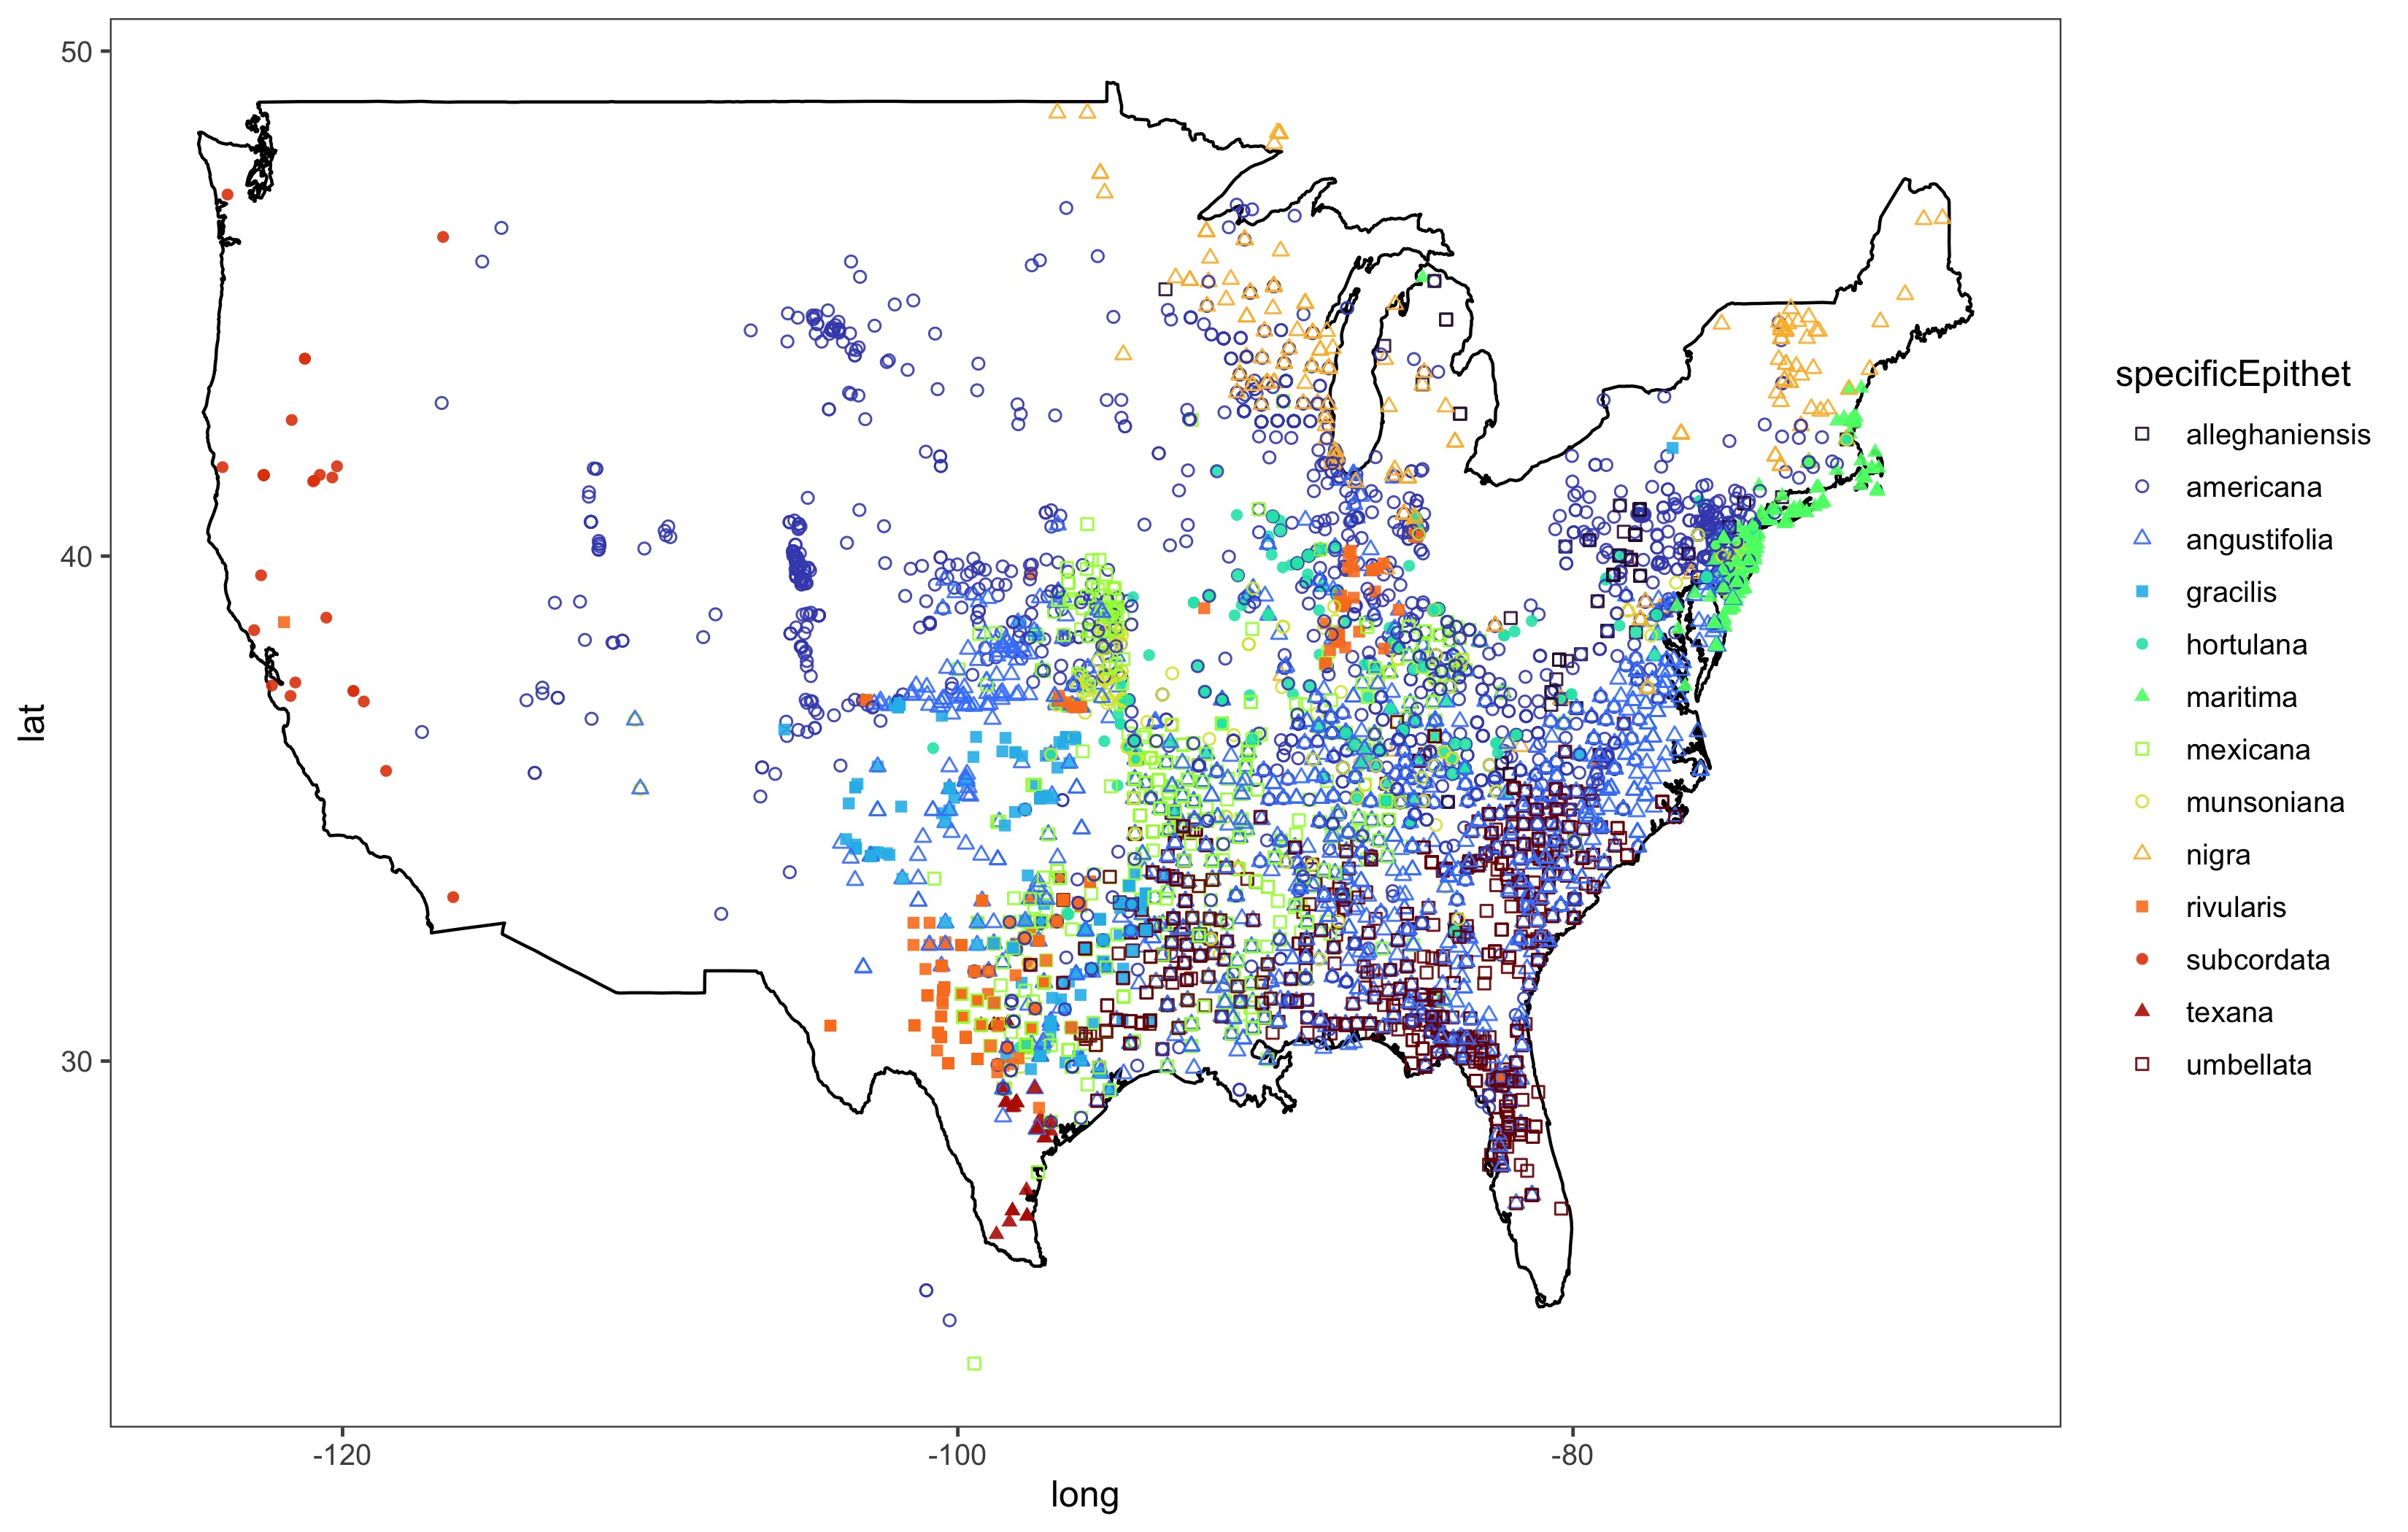
\includegraphics[width=\textwidth]{..//..//Plots/map.jpeg}
    \caption{Map to show where data come from and to point out the two never hysteranthy species are highly endemic}
    \label{fig:mappy}
\end{figure}

\begin{figure}[h!]
    \centering
 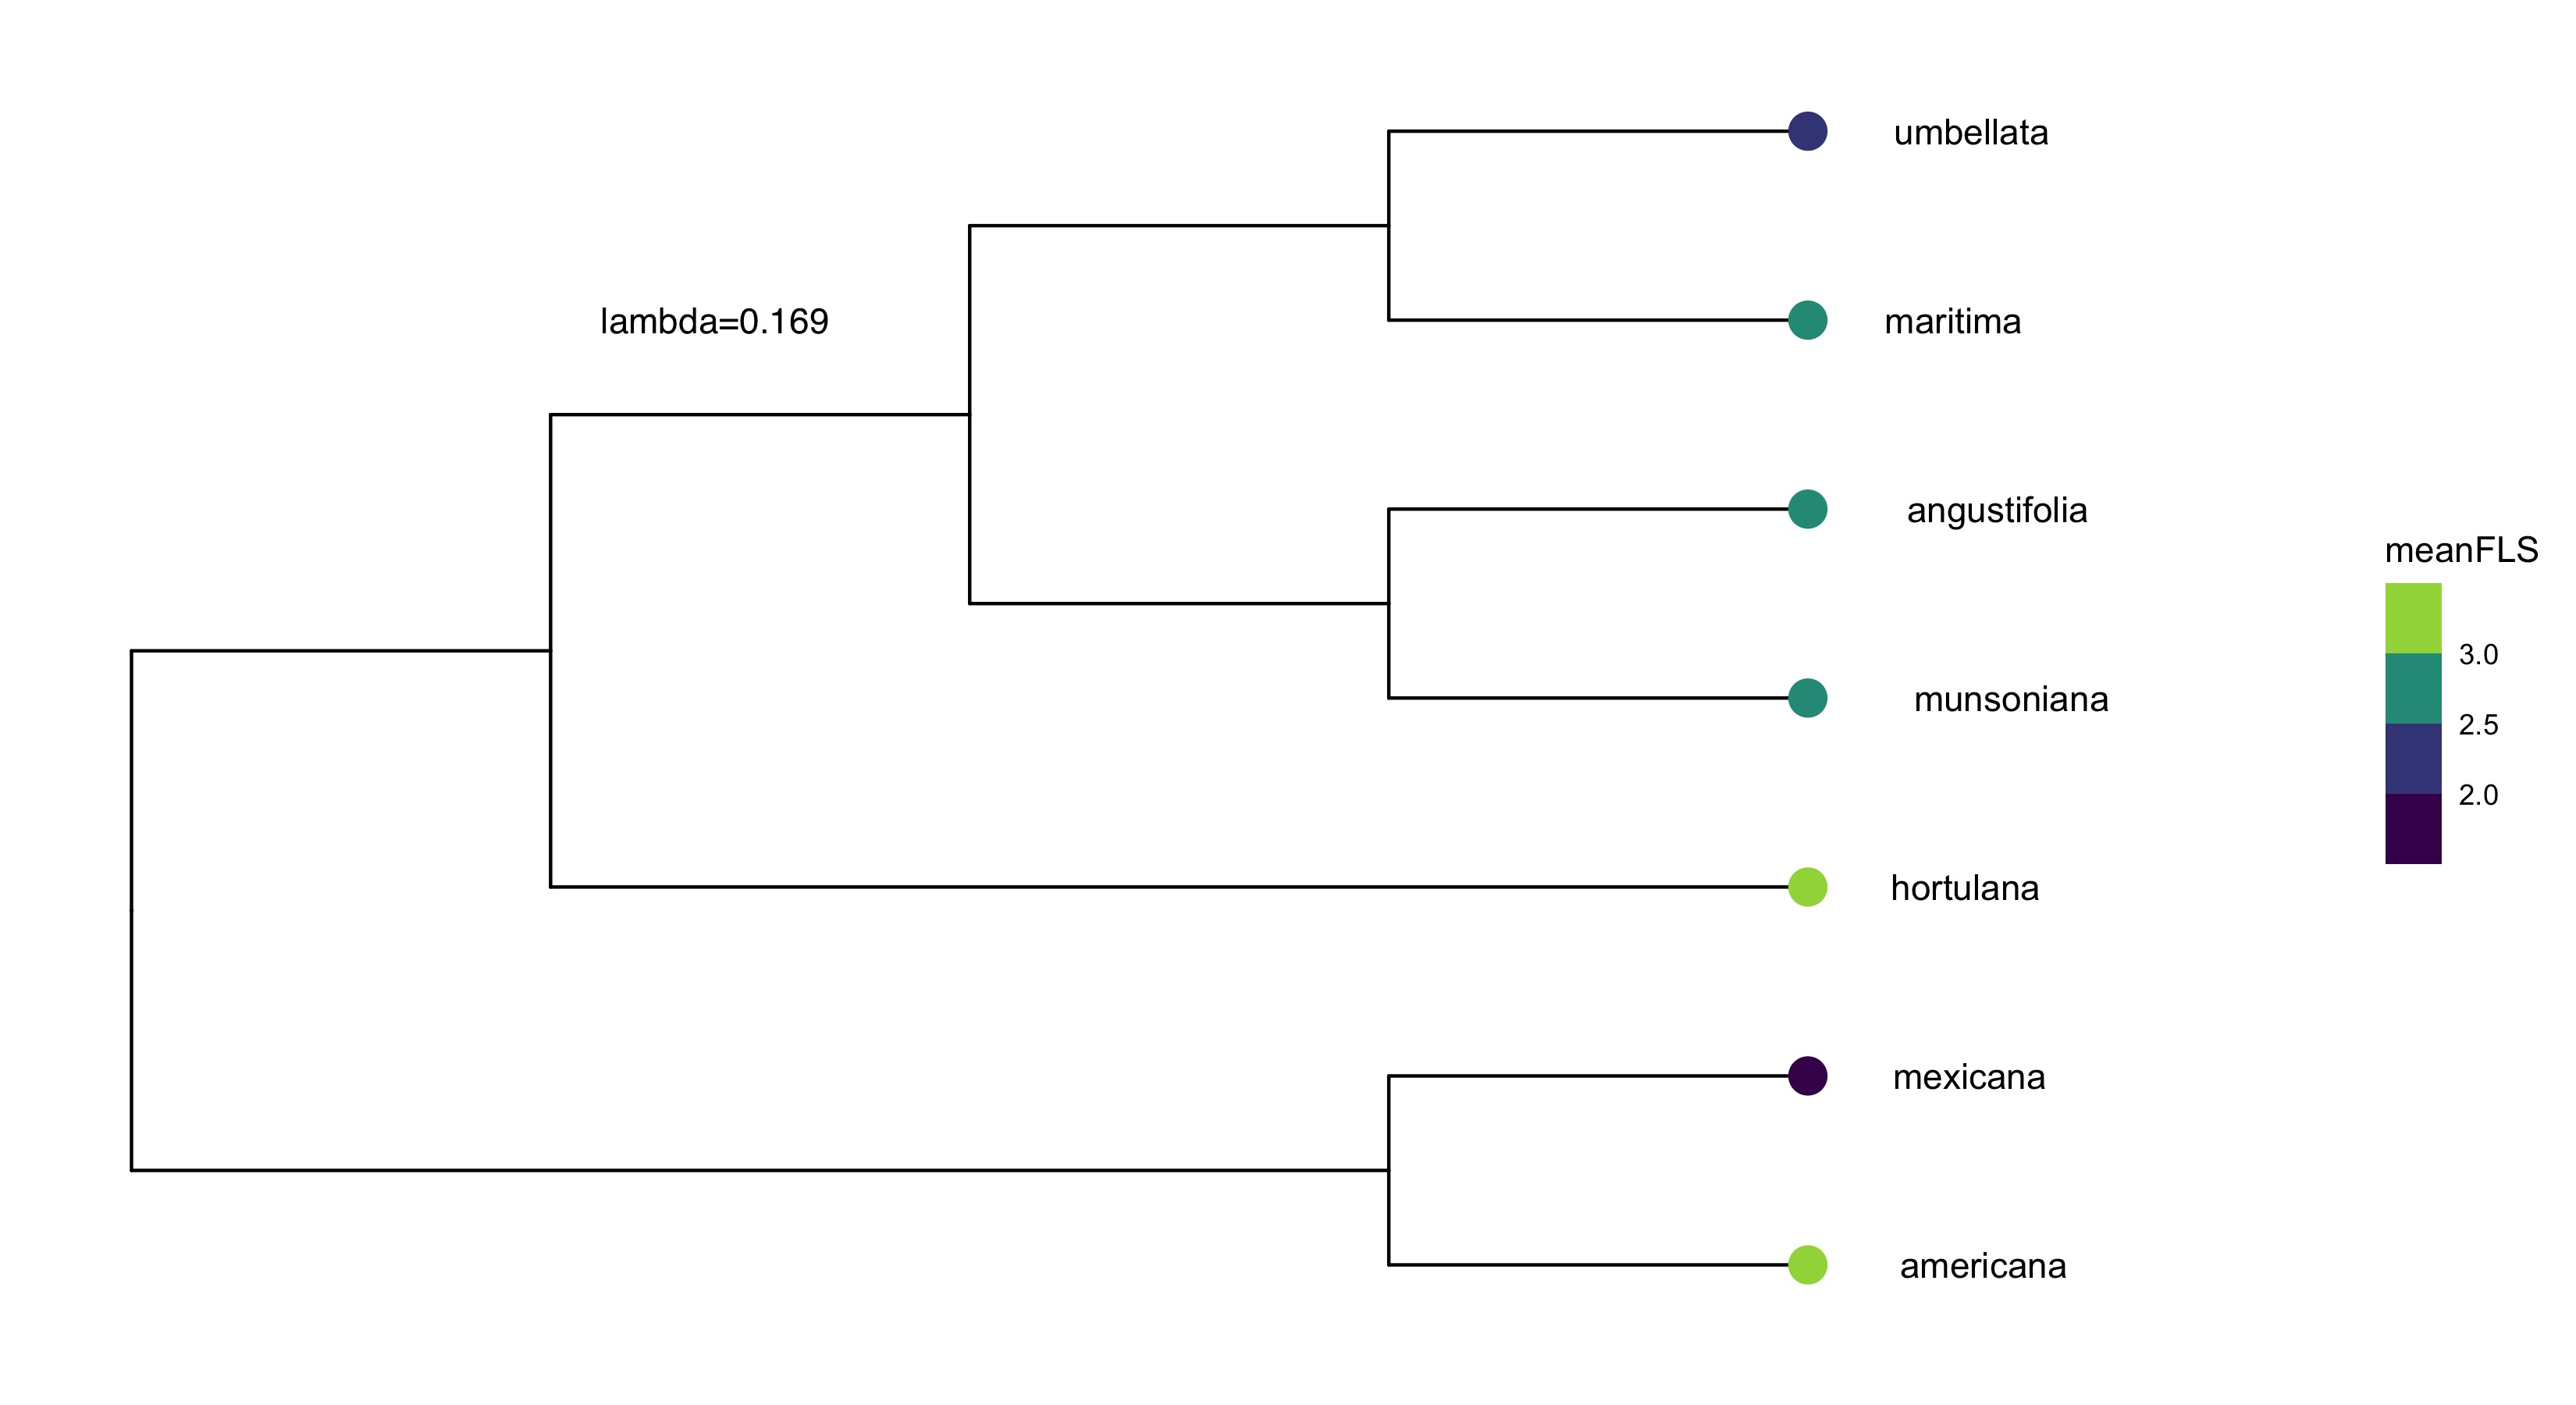
\includegraphics[width=\textwidth]{..//..//Plots/phylosig1.jpeg}
    \caption{place holder for the phylgenies: Ideally will have all N.A. Prunus \texit{and} Prunocerasus }
    \label{fig:phylo}
\end{figure}

\begin{figure}[h!]
    \centering
 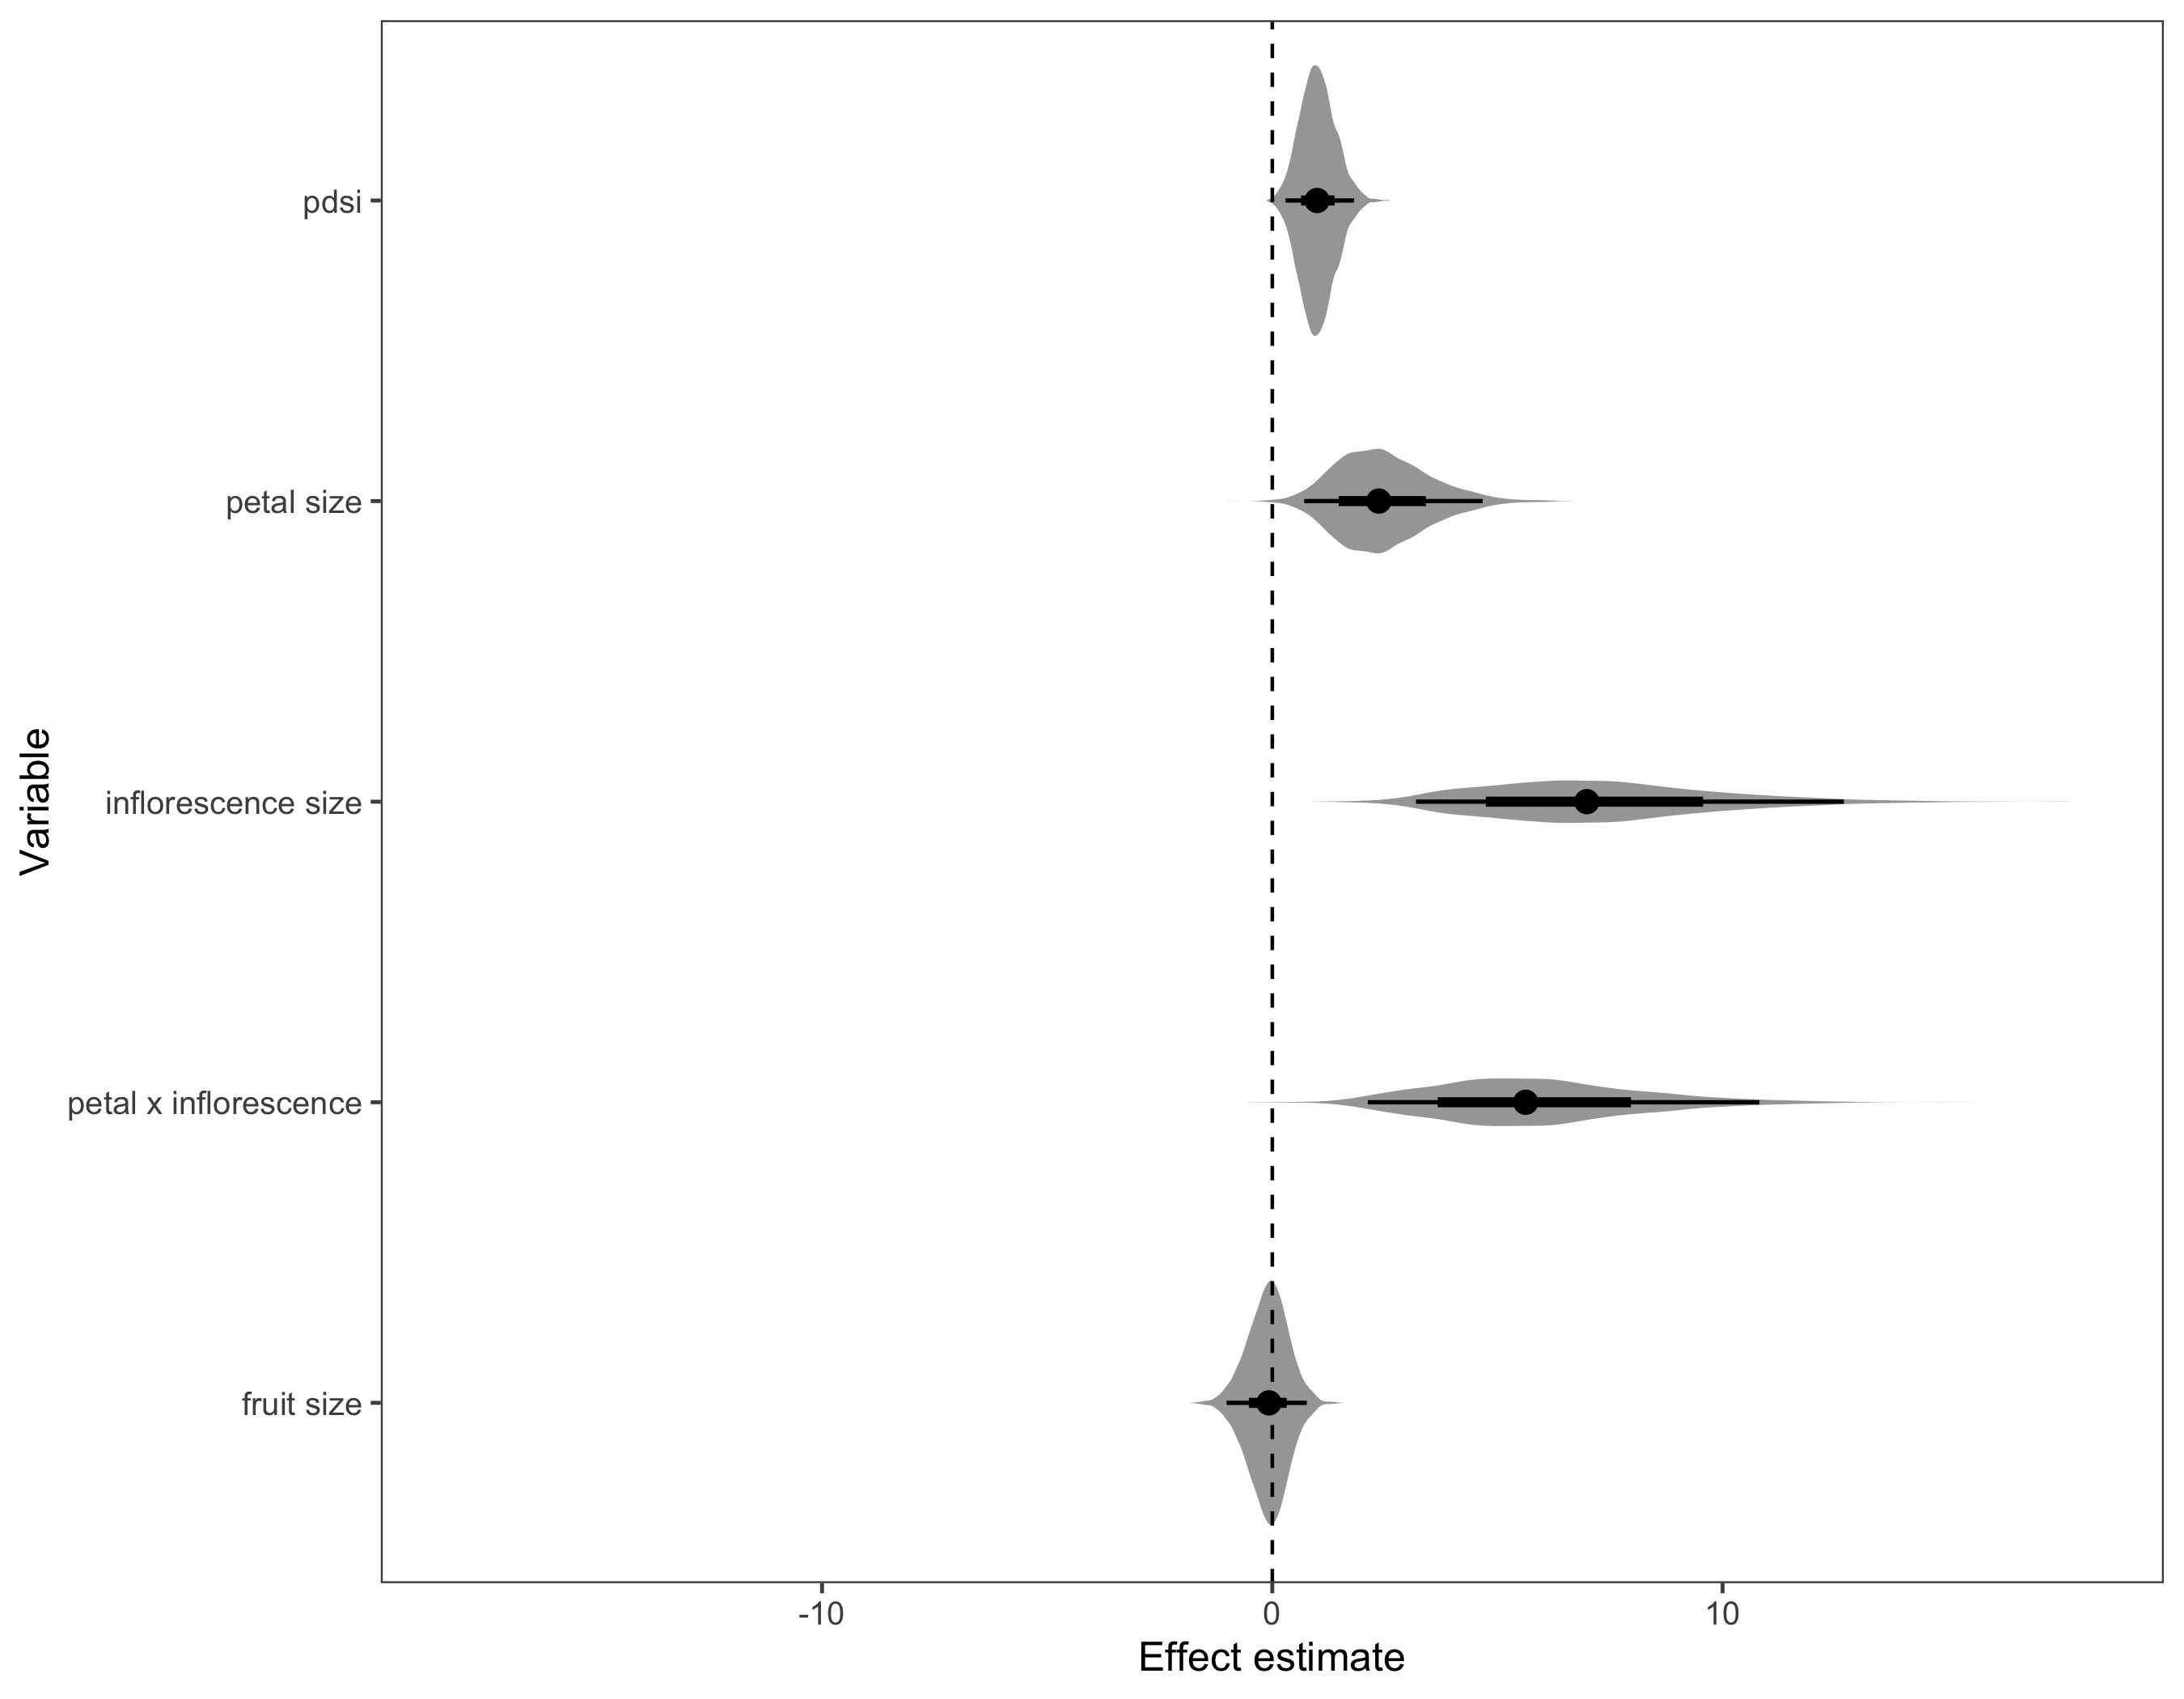
\includegraphics[width=\textwidth]{..//..//Plots/fullprunus_mus.jpeg}
    \caption{From the full genus analysis: Positive is less hysteranthus so aridity increases ihysteranthy, flower size decreases (ie smaller flowers- more hysteranthous) and no relationship with fruit size }
    \label{fig:cherries}
\end{figure}


\begin{figure}[h!]
    \centering
 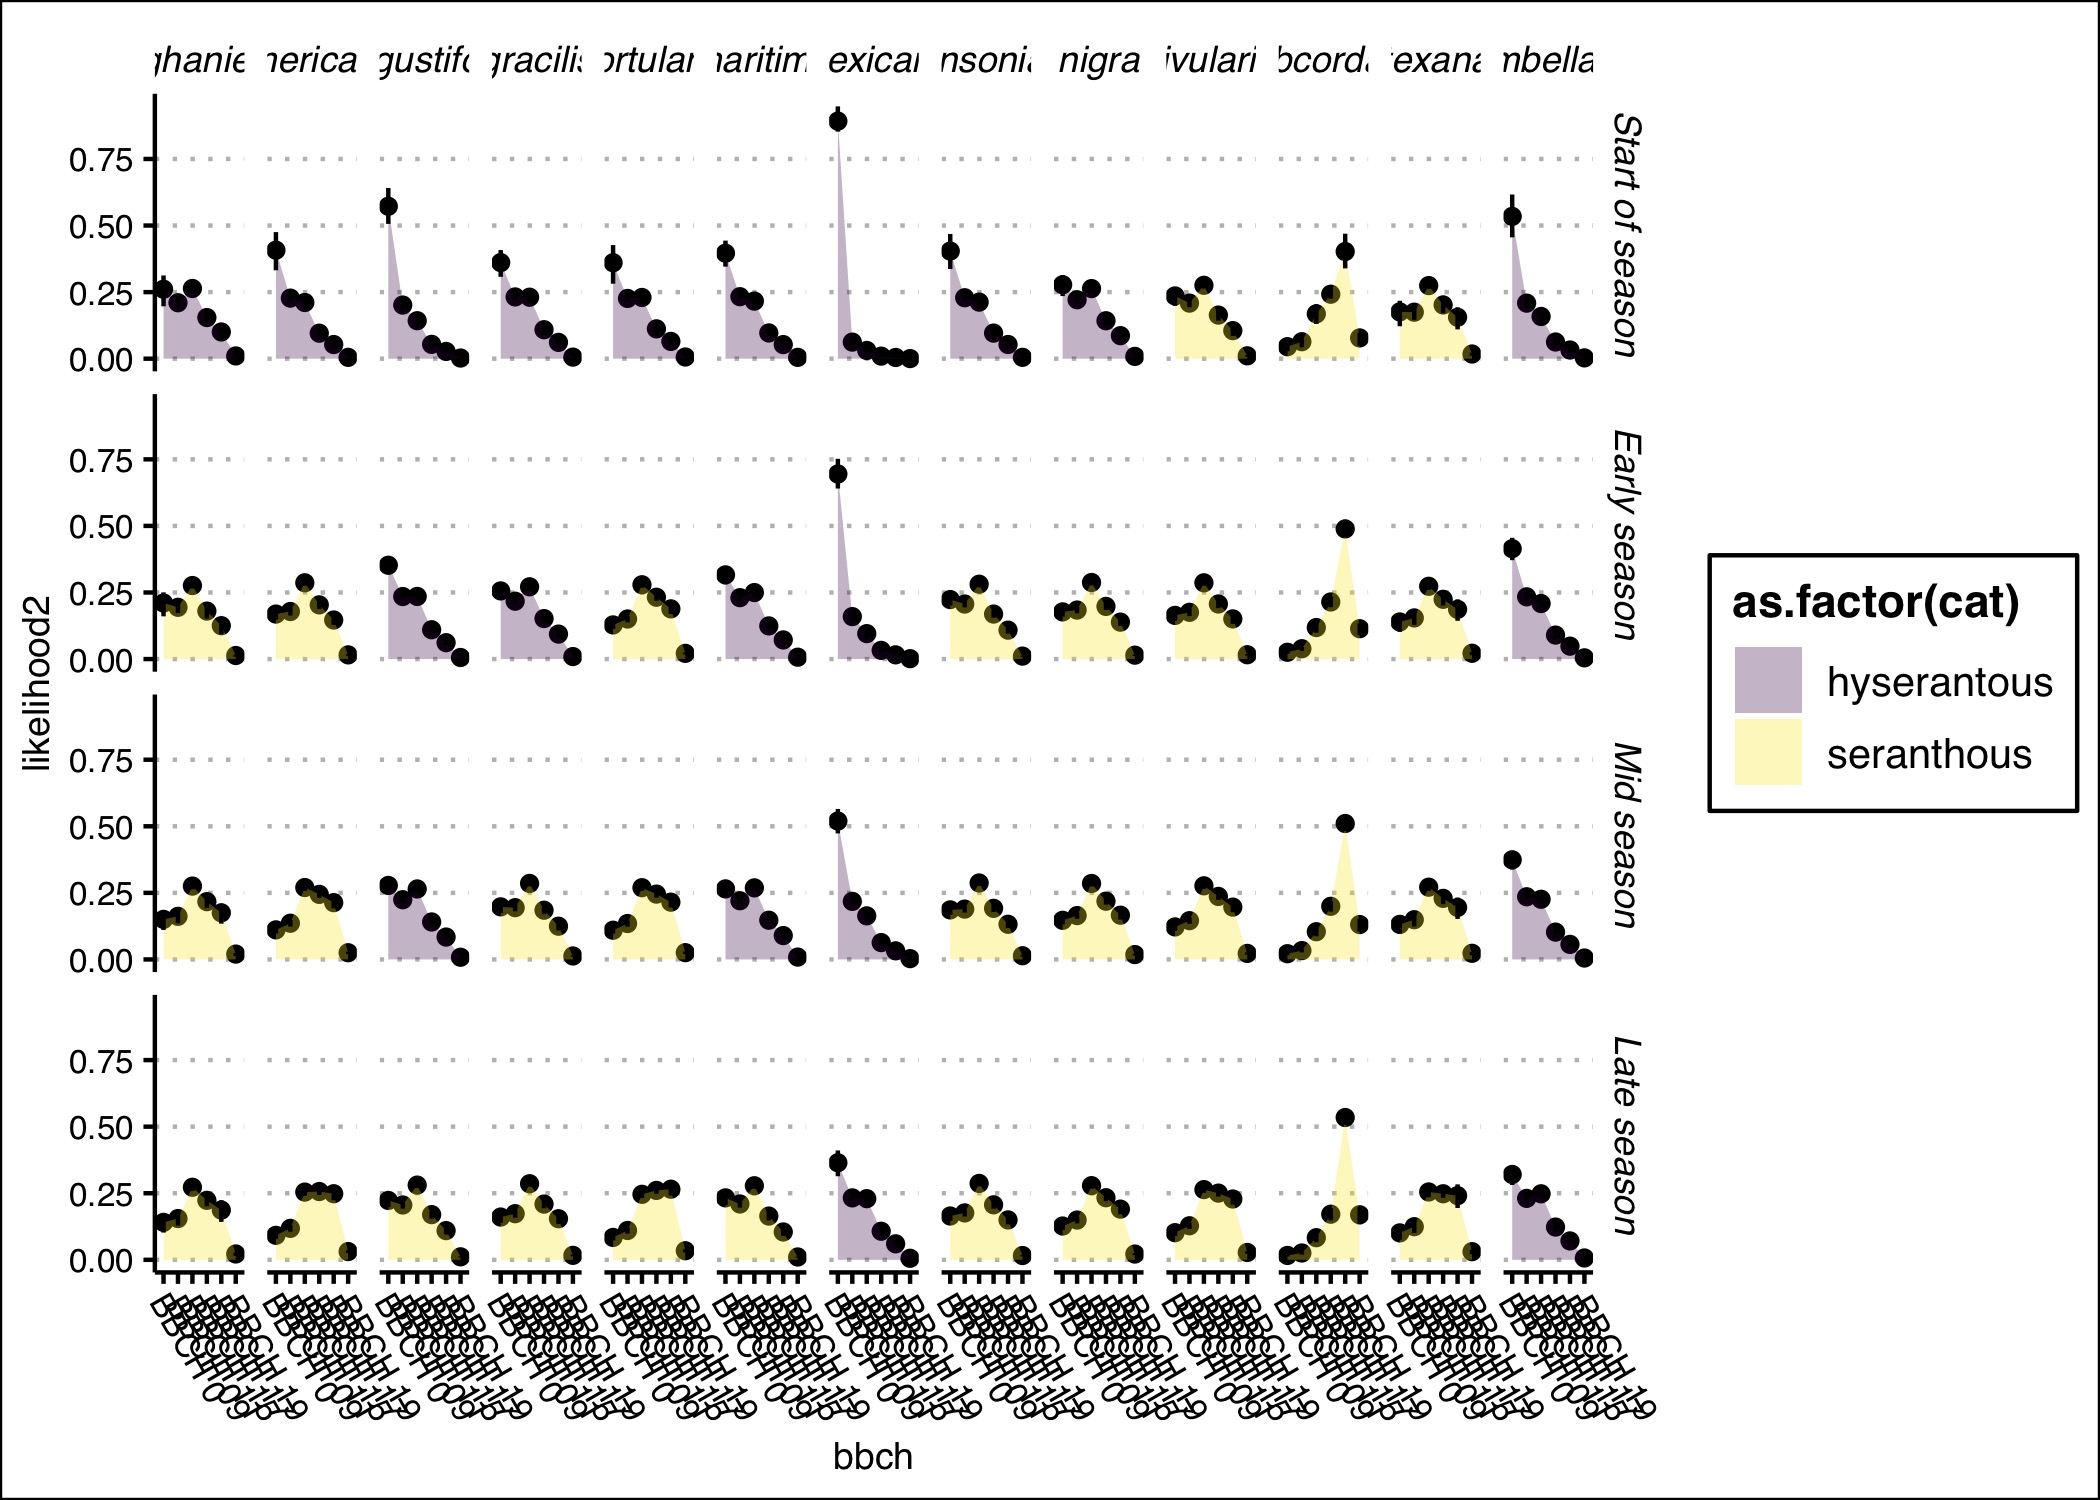
\includegraphics[width=\textwidth]{..//..//Plots/ord_quants.jpeg}
    \caption{ Likelihood of hysteranthy throughout the flowering season for each species in prunocerasus}
    \label{fig:plums}
\end{figure}

\begin{figure}[h!]
    \centering
 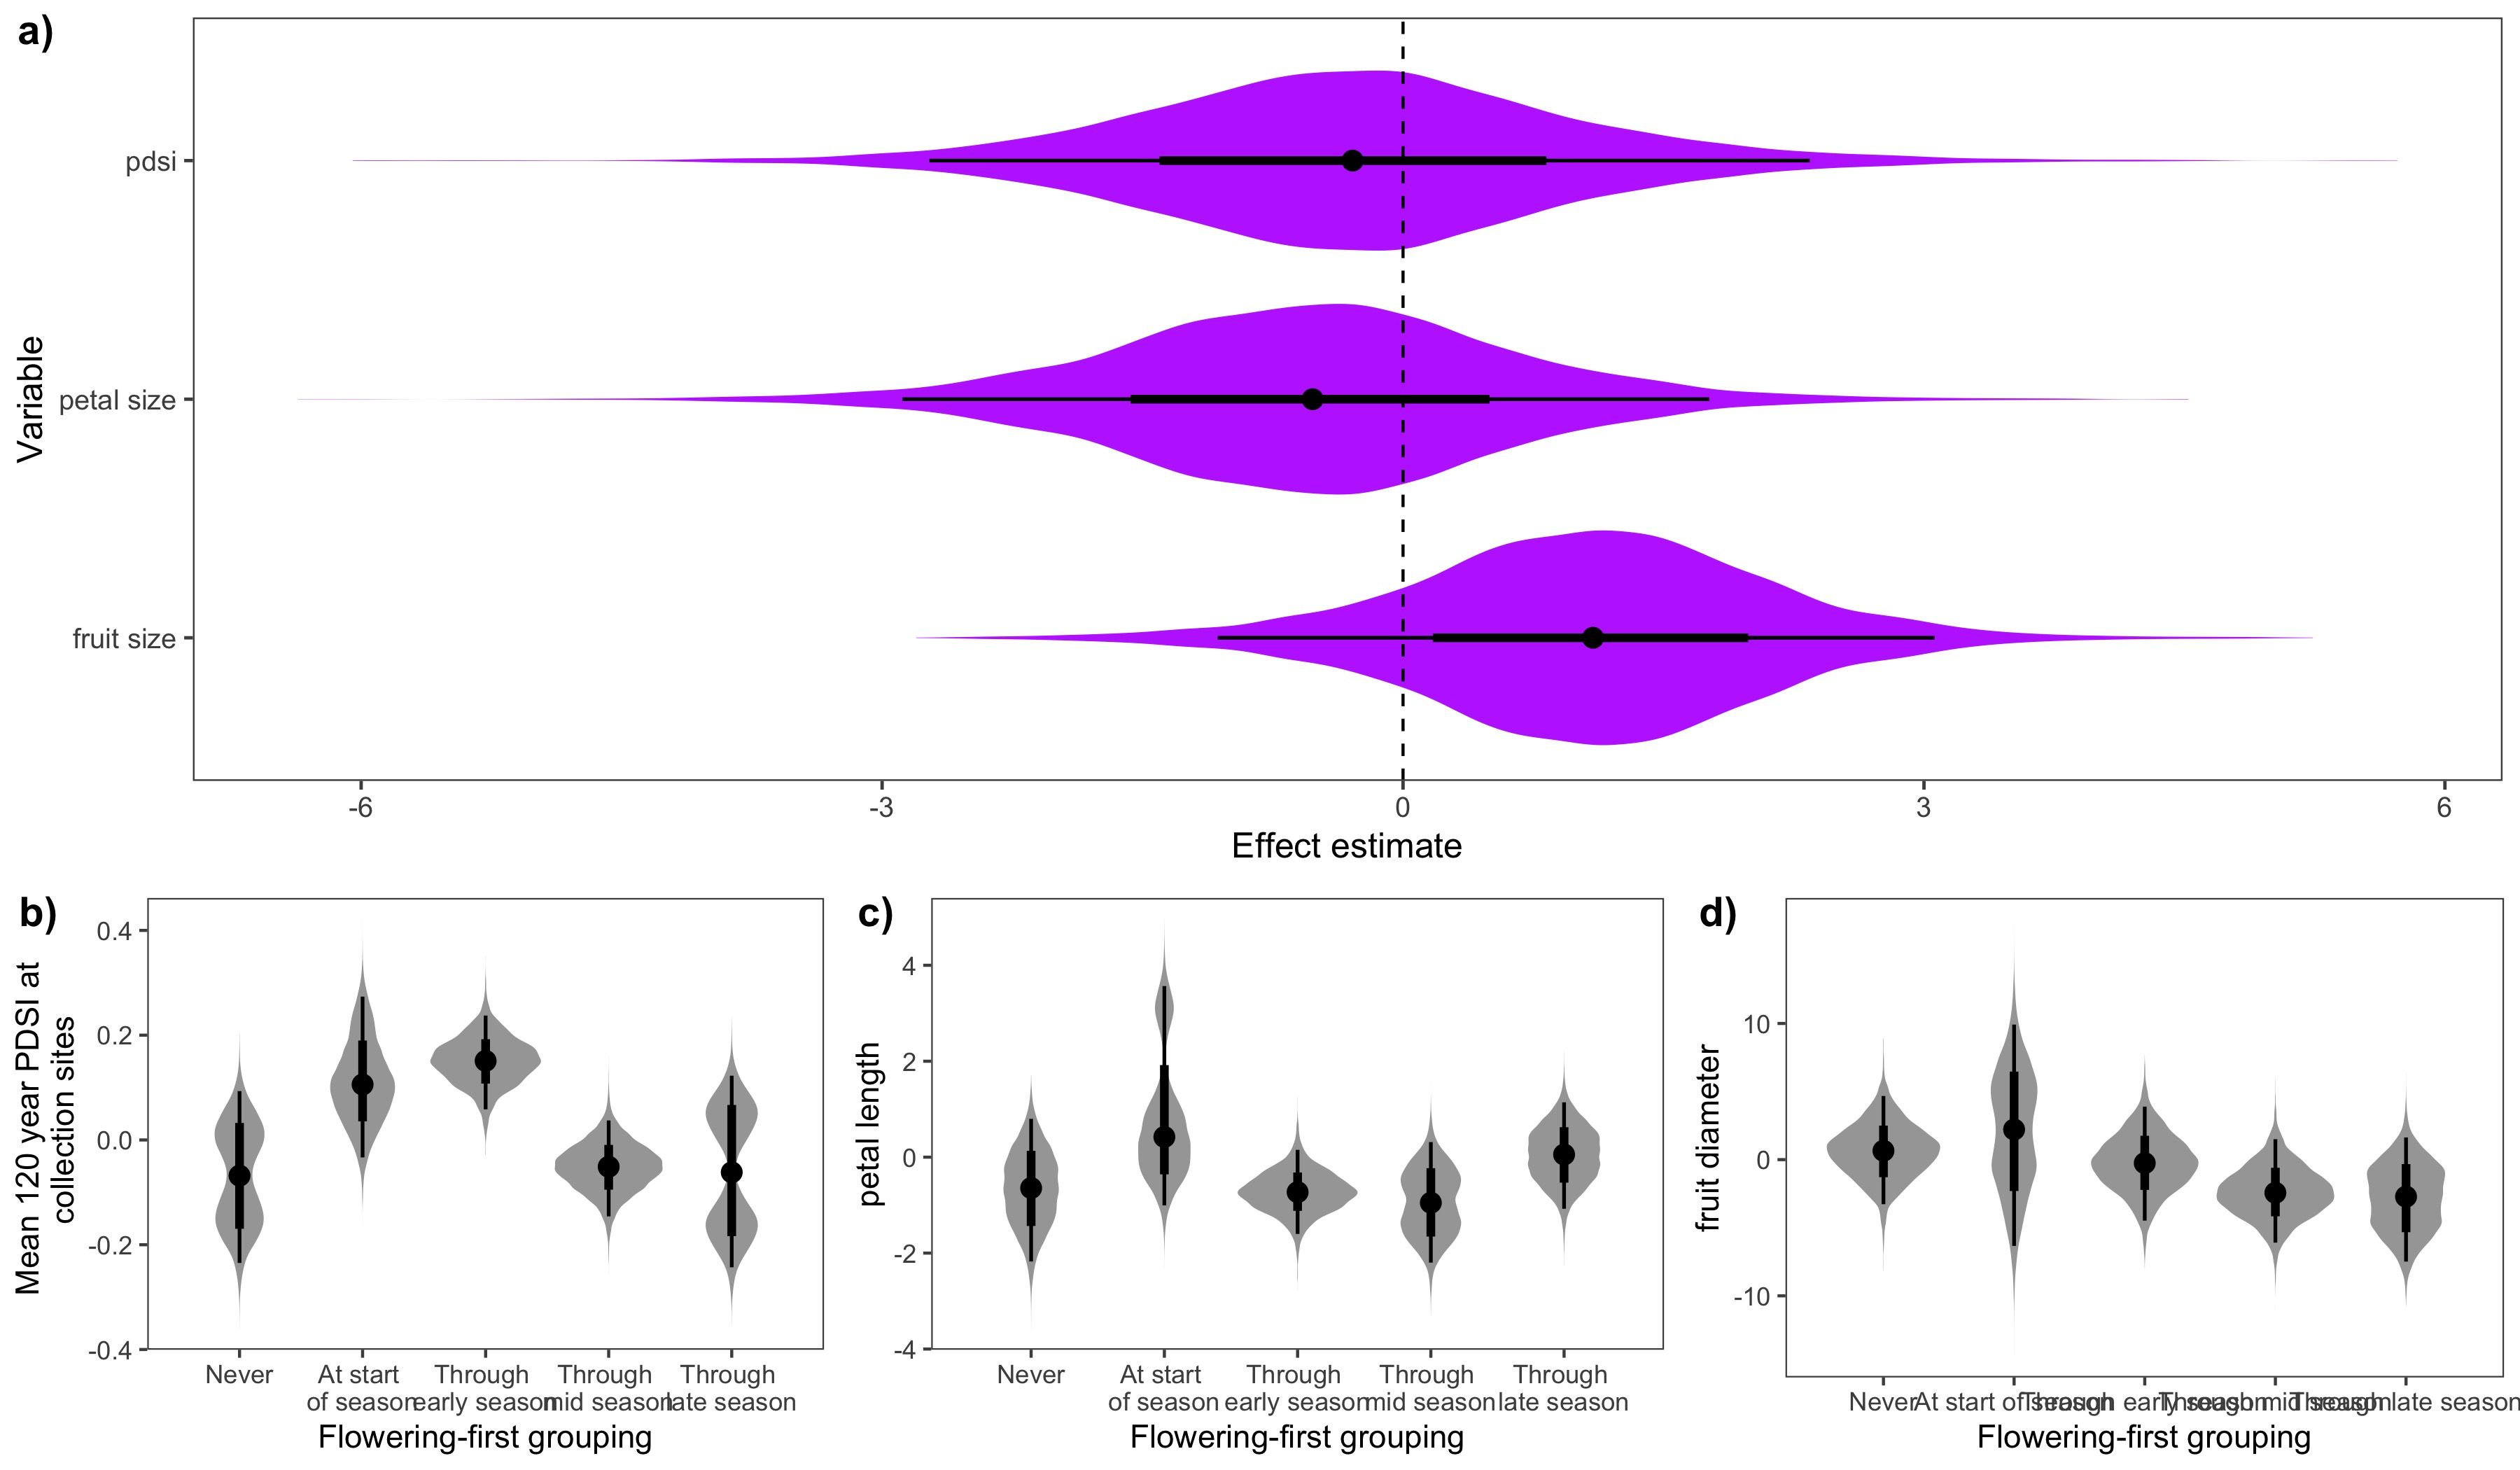
\includegraphics[width=\textwidth]{..//..//Plots/cerasus_mus.jpeg}
    \caption{Effect estimates. Why are they so different in prunucerasus? 1. measurement error model increases uncertainty. 2. outlyers have stronger influence. 3. Maybe too closely related (all flower to somedegree while leave are developing) }
    \label{fig:prunes}
\end{figure}


\begin{figure}[h!]
    \centering
 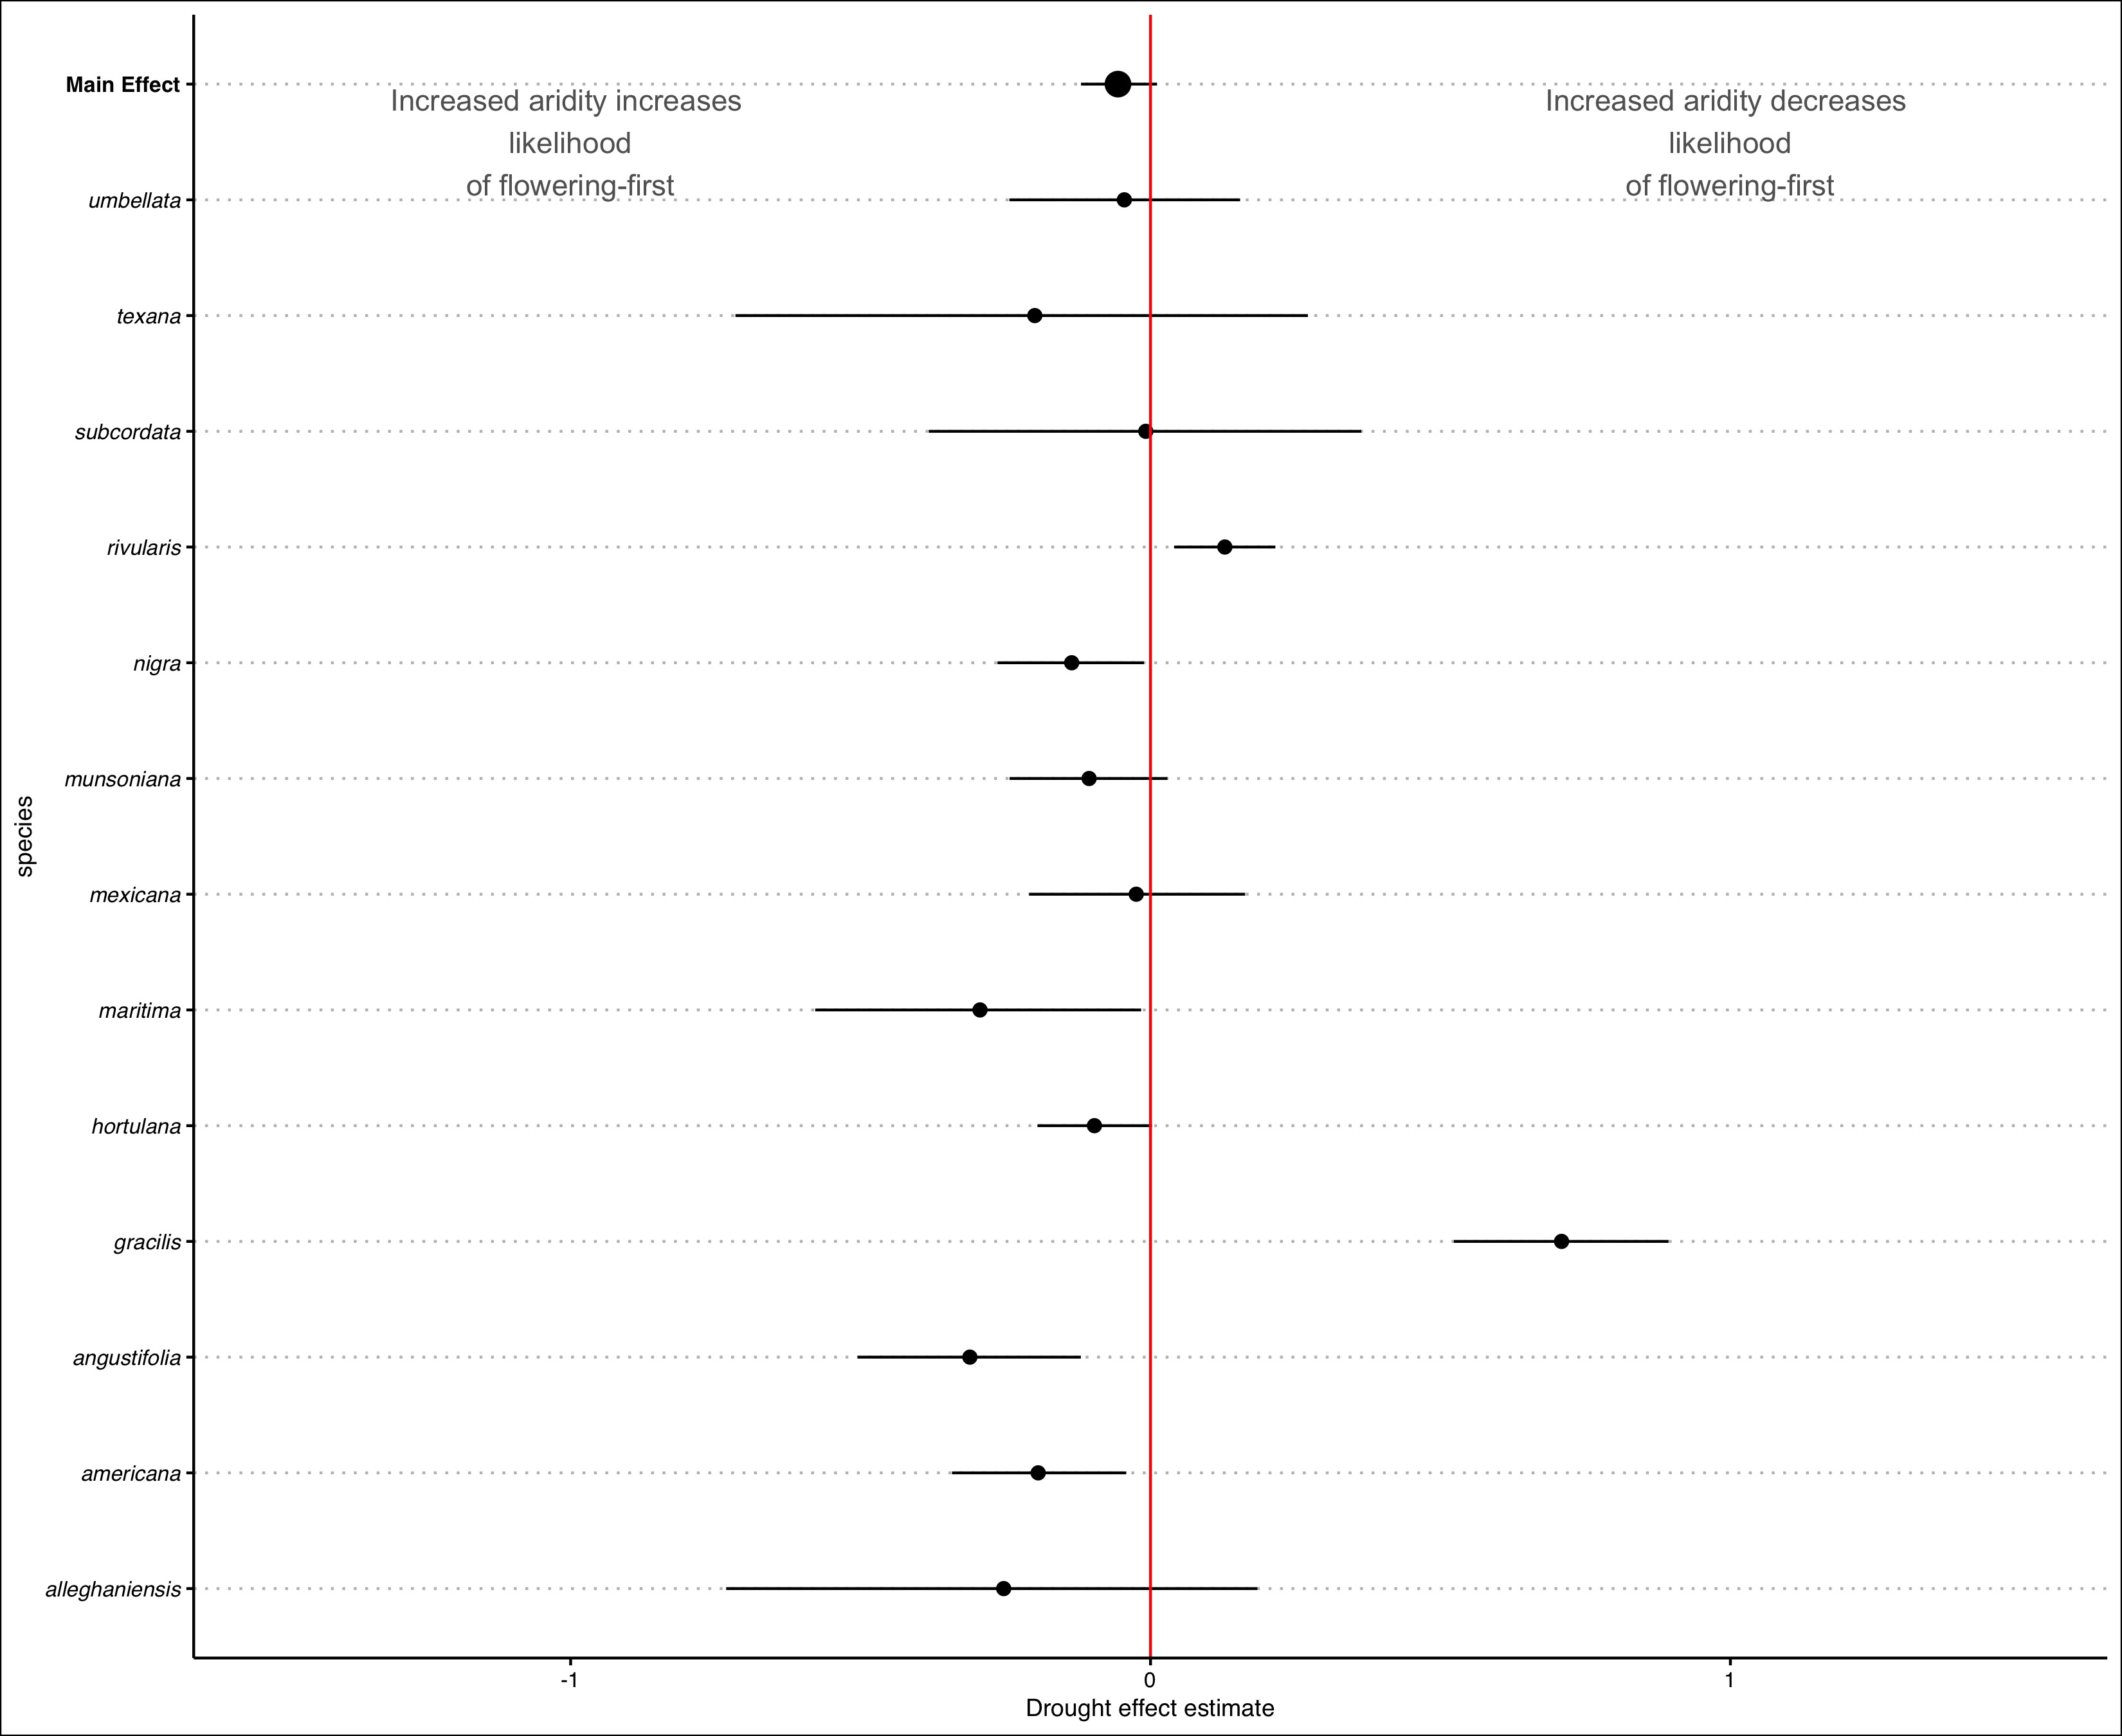
\includegraphics[width=\textwidth]{..//..//Plots/droughtstuff.jpg}
    \caption{Hysteranthy more likely in drought years.}
    \label{fig:plastic}
\end{figure}

\end{document}
